\documentclass[12pt,aspectratio=1610]{beamer}
%aspectratio=169 1610, 149, 54, 43 and 32
% There are many different themes available for Beamer. A comprehensive
% list with examples is given here:
% http://deic.uab.es/~iblanes/beamer_gallery/index_by_theme.html
% You can uncomment the themes below if you would like to use a different
% one:
%\usetheme{AnnArbor}
%\usetheme{Antibes}
%\usetheme{Bergen}
%\usetheme{Berkeley}
%\usetheme{Berlin}
%\usetheme{Boadilla}
%\usetheme{boxes}
%\usetheme{CambridgeUS}
%\usetheme{Copenhagen}
\usepackage[T1]{fontenc}
\usepackage[utf8]{inputenc}
\usetheme{Darmstadt}
%\usetheme{default}
%\usetheme{Frankfurt}
%\usetheme{Goettingen}
%\usetheme{Hannover}
%\usetheme{Ilmenau}
%\usetheme{JuanLesPins}
%\usetheme{Luebeck}
%\usetheme{Madrid}
%\usetheme{Malmoe}
%\usetheme{Marburg}
%\usetheme{Montpellier}
%\usetheme{PaloAlto}
\usetheme{Pittsburgh}
%\usetheme{Rochester}
%\usetheme{Singapore}
%\usetheme{Szeged}
%\usetheme{Warsaw}	

\usecolortheme{seahorse} %beetle, seahorse, wolverine, dolphin, beaver
\useoutertheme[subsection]{miniframes}
%smoothbars
%\useinnertheme{default}
\usepackage[francais]{babel}%
\usepackage{adjustbox}
%\usepackage[english]{babel}
%\usepackage{bookman}


\usepackage{lmodern}
\usepackage{scalefnt}
\usepackage{subcaption}
\setbeamertemplate{itemize items}[triangle]

%
\usefonttheme[structurebold]{}
%{serif}
%\mode<beamer>{\setbeamertemplate{blocks}[rounded][shadow=true]}
%\setbeamertemplate{caption}[numbered]


\captionsetup{compatibility=false}

% or whatever

\usepackage{pdfpages}
\usepackage{changepage}
\usepackage{pdflscape}
\usepackage{xspace}
\usepackage{graphicx}
\usepackage[xcolor]{}
\usepackage{adjust box}
\usepackage[T1]{fontenc}
%\usepackage[utf8]{inputenc}
\usepackage{etex}
\usepackage{tikz}
\usepackage{booktabs,caption,fixltx2e}
\usepackage[flushleft]{threeparttable}
\usepackage{tabularx}
\usepackage{endnotes}
\usepackage{eurosym}
\usepackage{multirow}
\usepackage{comment}
\usepackage{pst-grad} % For gradients
\usepackage{pst-plot} % For axes
\usepackage{physics}
\usetikzlibrary{positioning,decorations.pathreplacing,shapes}
\usetikzlibrary{snakes}
\usetikzlibrary{calc}
\setbeamertemplate{navigation symbols}{} % Helps get rid of navigation symbols
\setbeamertemplate{footline}[frame number]
%\usepackage{beamerthemesplit}


\title[Intro Stat \& Proba] % (optional, use only with long paper titles)
{\bf Apprentissage statistique supervisé}

\subtitle
{La Régression Logistique} % (optional)

\author[]{Dr. Modeste Dayé} % (optional, use only with lots0 of authors)
{  }
% - Use the \inst{?} command only if the authors have different
%   affiliation.

%\institute[Universities of Somewhere and Elsewhere] 
%{\textbf {TSE}}




\institute[]{ \textbf{EEIA 2023}\\  \textit{}}
	
	
	\AtBeginSection[]
	{
		\begin{frame}<beamer>
			\frametitle{Plan}
			\tableofcontents[currentsection]
		\end{frame}
	}
	
\begin{document}

\begin{frame}
  \titlepage
 \end{frame}

\section*{}
\tableofcontents


\section{Motivation}
\subsection{}

\begin{frame}
	
	\textcolor{blue}{Prédiction ou explication d'une variable cible}
	
	\begin{itemize}
		\item Dans un jeu de données contenant  une variable (cible) d'intérêt (continue ou catégorielle) et des caractéristiques pertinentes qui lui sont liées :
		 $ \textcolor{blue}{y= f(X) + \epsilon}$
		
		\begin{itemize}
			\item Exercice de prédiction de y
			\item Exercice d'explication de la mesure dans la quelle chacune des caractéristiques affecte $y$ et sa pertinence lorsqu'on rapporte à la population: inférence statistique;
		\end{itemize}
		
			
		
		\item Dans les 2 cas, on veut comprendre le processus de génération des données: quelle est la logique qui lie les caractéristiques à la variable cible: est-ce une logique linéaire, non-linéaire, paramétrique, non-paramétrique ?
		
	\begin{itemize}
		\item Il faut pouvoir utiliser un bon algorithme, et faire usage de la théorie liée au domaine (modèle économique, voir littérature économique) pour bien choisir son $f()$ ou ne même pas en imposer.
	\end{itemize}
		
	\end{itemize}
\end{frame}
\begin{frame}
	\begin{figure}
		\centering
		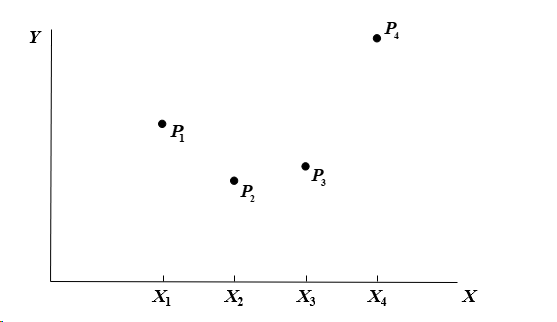
\includegraphics[width=0.9\linewidth]{scatterplot}
	\end{figure}
\end{frame}	

\begin{frame}
	\begin{figure}
		\centering
		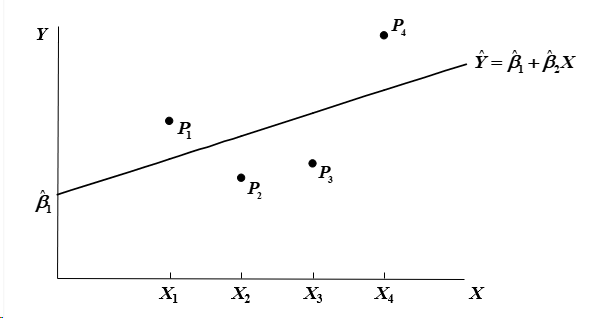
\includegraphics[width=0.9\linewidth]{ajustement}


	\end{figure}
	
\end{frame}



\begin{frame}
	\begin{figure}
		\centering
		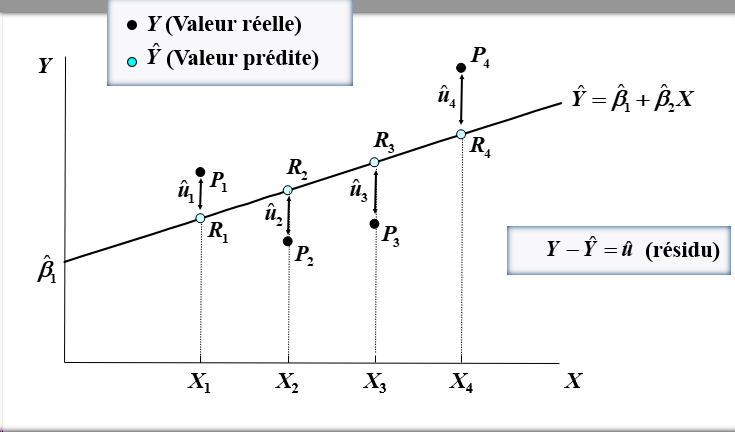
\includegraphics[width=0.9\linewidth]{residuspng}
	\end{figure}
	
\end{frame}

\begin{frame}
	\textcolor{blue}{\textbf{\large Régression}  \\
	Objectif : On veut comprendre la variance, i.e. les différentes valeurs prises par une \textbf{variable continue à partir d'une ou de plusieurs caractéristiques}} 
	\vspace{0.5 cm}
	\begin{itemize}
		\item Cas simple: Régression linéaire simple: 	$$ y_i=\beta_0+\beta_1x_i+\epsilon_i $$, 
		
		\item Moindre Carrées Ordinaires (MCO) : meilleur adjustment possible d'un nuage de points entre variables continues: $\displaystyle\min  
		\sum_{i=1}^{n}\hat{u}^2_i=(y_i-\hat{y}_i)^2$
		\item y continue 
	\end{itemize}
\end{frame}




\begin{frame}
		\textcolor{blue}{\textbf{\large Questions de classification}}
	\begin{itemize}
		\item<1-> Certains 	\textcolor{blue}{poursuivent leurs études} après le bac \textcolor{blue}{d'autres pas}. 
		\begin{itemize}
			\item <1->	\textit{Nous disposons des caractéristiques des élèves réussissant au bac  (age, notes en classe et au bac, caractéristiques socio-démographiques des parents, etc.)}
			
			\item<2-> Peut-on construire un modèle qui nous dise les chances qu'un nouveau bachelier aille à l'université (ou dans  une filière spécifique)? Autrement dit, classer les nouveaux bacheliers.
			
		\end{itemize}
		
		\vspace{0.5cm}
		
		
		\item <3-> Certaines 	\textcolor{blue}{candidatures ont été retenues} pour l'EEIA 2023 et 	\textcolor{blue}{ d'autres pas}.
		
		\begin{itemize}
			\item \textit{Peut-on prédire la probabilité d'être sélectionné (au moins pour la phase entretien) d'un candidat à l'EEIA 	étant données ses caractéristiques  et la qualité de la LM (plagiat éliminatoire) ?}  
			
			\item Les formateurs  de l'EEIA qui passent de nombreuses heures à lire les LM et discuter/creuser les motivations présentées par les candidats  seront sans doute intéressés.
			
		\end{itemize}
		
		
	\end{itemize}
	
\end{frame}



\begin{frame}{}
	
	\begin{itemize}

		\item Les variables binaires sont composées de 2 catégories: Oui/Non, malade/non-malade, admis/non-admis, etc.
		%Par exemple : \textcolor{blue}{l'apprenant EEIA 2023 a t-il déjà étudié la régression logistique par le passé?} %étant données ses caractéristiques (niveau d'études, expérience pro, domaine d'études, etc.)?} 
		\\
		$\Rightarrow$ Deux réponses possibles : Non/Oui, que l'on pourra encoder dans une variable binaire numérique  0/1 pour exploitation dans les algorithmes de classification.

	\end{itemize}
	
\end{frame}


	\section{Classification: Modèles de probabilité}
\begin{frame}
		\textcolor{blue}{\textbf{\large Le Modèle de Probabilité Linéaire (MLP) }}
		\begin{itemize}
			

		\item Soit le modèle linéaire simple  : 
	$$ y_i=\beta_0+\beta_1x_i+\epsilon_i, \text{pour un individu i} $$
	où : 
	
	\begin{itemize}
		\item $y_i$ :  Variable à expliquer (cible ou \textit{target}) qui prend la valeur 1 si l'apprenant  $i$ avait déjà étudié la régression logistique par le passé et 0 sinon.
		\item $x_i$ :  le domaine de formation de l'apprenant  $i$ (variable catégorielle ici: stat, maths, info, agronomie, etc...)
		\item $\epsilon_i$ l'erreur de spécification du modèle (terme d'erreur)
		\item $\beta_0$ et $\beta_1$ sont les paramètres à estimer et qui permette de comprendre le processus de génération des données ($y_i$).
	\end{itemize}
	
	\end{itemize}
	
\end{frame}


\begin{frame}{}
%	\item MCO: $\Rightarrow$ MXZZZZC              Wzodèle de probabilité linéaire (MLP)

\centering 	$ y_i=\beta_0+\beta_1x_i+\epsilon_i $
	
	Avec un modèle linéaire et une variable cible dichotomique, on prédit des probabilités: 
	\begin{itemize}

		\item Si on respecte l'hypothèse d'espérance nulle du terme d'erreur ($E(\epsilon_i/x_i)=0$) alors $E(y_i/x_i)=\beta_0+\beta_1x_i$
		
		\item On peut réécrire cette espérance sous forme de probabilité.
		Soit $p_i$ la probabilité que $y_i=1$ alors $(1-p_i)$ est la probabilité que $y_i=0$ \\
		
		On a : 
		$$ E(y_i/x_i)=1 \times p_i + 0 \times (1-p_i)=p_i=\beta_0+\beta_1x_i$$
		D'où le fait qu'on parle de Modèle linéaire de probabilité:
		
$$\hat{p_i}(y_i=1/x)=\hat{\beta_0}+\hat{\beta_1}x_i$$
	\end{itemize}
\end{frame}


\begin{comment}
	\begin{frame}{}
		\begin{itemize}
			
			\item Le codage de la variable expliquée en 0/1 est par ailleurs parfaitement arbitraire, nous aurions très bien pu la coder sous la forme de 0/10.
			\item Nous devons respecter le fait que $0 \le p_i=\beta_0+\beta_1x_i \le 1$ ce qui peut ne pas être le cas suivant les données
			\item Nous pouvons avoir un effet de seuil :  à partir d'une certaine valeur de $x$ la probabilité d'occurence de $y$ ne va pas augmenter (ou très peu) 
		\end{itemize}
		
		
	
	\end{frame}
\end{comment}




\begin{frame}
	
	MLP: $$\hat{p_i}(x)=\hat{\beta_0}+\hat{\beta_1}x_i$$
	
\pause
	Problème: p $\in [0, 1]$ alors que: $$\hat{\beta_0}+\hat{\beta_1}x_i \in R$$
	
	Idée:  trouver une transformation $\phi~de~ p_i(x)$ telle que $\phi(p_i(x))$ prenne 	ses valeurs dans $R$.
	
	\begin{equation*}
		\phi(\hat{p_i}(x))= \hat{\beta_0}+\hat{\beta_1}x_i
	\end{equation*}
	
\end{frame}



\begin{frame}{}
	
	\textcolor{blue}{\textbf{\large Prédictions MLP parfois abérrantes}}
	(Voir TP plus tard)
	\begin{figure}
		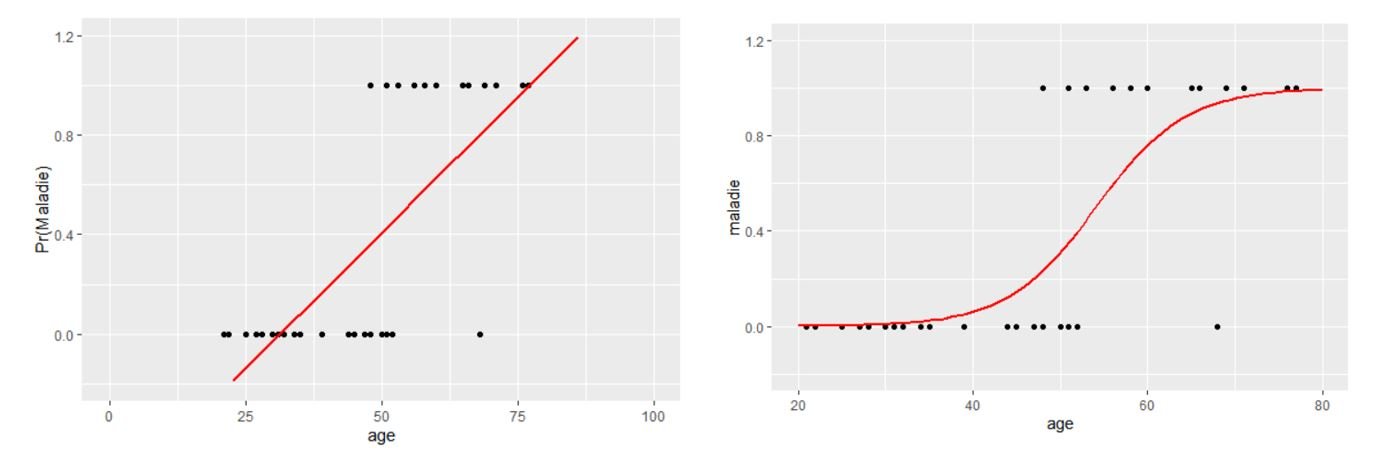
\includegraphics[scale=0.52]{lin_logistic.JPG}
		
		\label{}
	\end{figure}
\end{frame}




\begin{frame}
	
	\textcolor{blue}{\large Modélisation par les CDF: fonctions de répartition}
	\vspace{0.5cm}
	
	$$\hat{p_i}(y_i=1/x)=\hat{\beta_0}+\hat{\beta_1}x_i$$
	
	Nous souhaitons que  : 
	\begin{itemize}
		\item $E(y_i/x_i)=p_i$ soit compris entre 0 et 1
	\end{itemize}
	
	Deux modélisations sont utilisées en économétrie/statistique  : 
	\begin{itemize}
		
		\item Probit (CDF, loi normale)
		\item \textbf{Logistique (CDF, loi logistique)}
		
	\end{itemize}
	
	\begin{equation*}
	\large 	F(z)=\frac{e^{z}}{1+e^{z}}
	\end{equation*}
		avec $z$ la variable aléatoire suivant une distribution logistique.
\end{frame}


\begin{frame}

		\begin{figure}
			\centering
			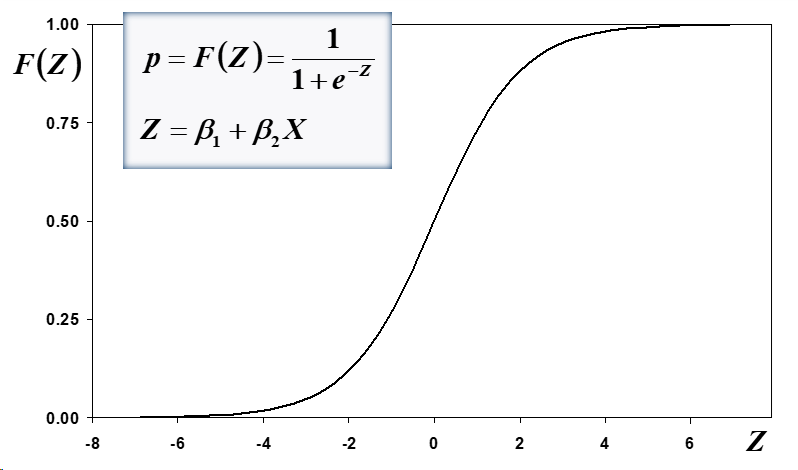
\includegraphics[width=0.9\linewidth]{logit1}
		\end{figure}
		
	
\end{frame}



\begin{frame}
	\begin{figure}
		\centering
		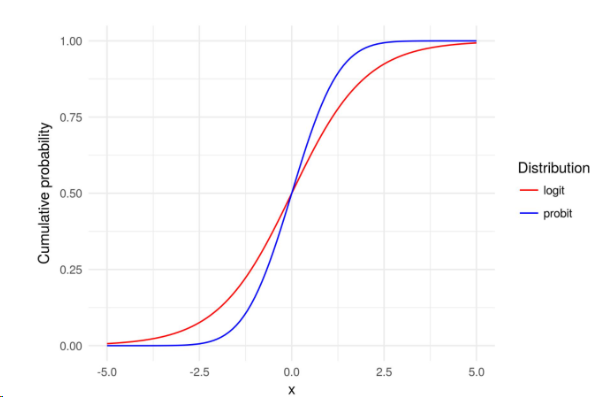
\includegraphics[width=0.85\linewidth]{logit_probit}
		\caption{}
	\end{figure}
	
\end{frame}



\begin{frame}
\textcolor{blue}{\large Régression Logistique}
		$$\hat{p_i}(y_i=1/x)=\hat{\beta_0}+\hat{\beta_1}x_i$$
La régression logistique modélise donc : $p_i(x)=\dfrac{exp(\beta_0+\beta_1x_i)}{1+exp(\beta_0+\beta_1x_i)}$





Avec 
	
	\begin{itemize}
		\item$\lim\limits_{z_i \rightarrow +\infty} p_i=1$
		
		\vspace{0.4cm}
		\item $\lim\limits_{z_i \rightarrow -\infty} p_i=0$
	\end{itemize}

	Où : $z_i=\beta_0+\beta_1x_i$
	

\end{frame}





\begin{frame}
	\textcolor{blue}{\large Régression Logistique}
	
	$$\hat{p_i}(y_i=1/x)=\hat{\beta_0}+\hat{\beta_1}x_i$$
	
	La régression logistique définit
	\begin{itemize}
		\item  $p_i(x)=\dfrac{exp(\beta_0+\beta_1x_i)}{1+exp(\beta_0+\beta_1x_i)}=\dfrac{1}{1+exp(-(\beta_0+\beta_1x_i))}$
		
	
	\pause
		\item 	 
		Et donc 	
		
		$ 1-p_i(x)=1-	\dfrac{1}{1+exp(-(\beta_0+\beta_1x_i))}=\dfrac{exp(-(\beta_0+\beta_1x_i))}{1+exp(-(\beta_0+\beta_1x_i))}$
		
		\pause 
		\item $\dfrac{p_i}{1-p_i}=exp(\beta_0+\beta_1x_i)$
	\end{itemize}
	
\end{frame}




\begin{frame}
		\textcolor{blue}{\large Régression Logistique}
	\begin{itemize}
		\item on a: $\dfrac{p_i}{1-p_i}=exp(\beta_0+\beta_1x_i)$ \pause \textbf{odds}: proba (chances) d'observer y=1 par rapport à y=0 pour une caractéristique x donnée. 
		\pause
		\item $log(\dfrac{p_i}{1-p_i})=\beta_0+\beta_1x_i$ avec  $log(\dfrac{p_i}{1-p_i})$, 	\textcolor{blue}{la fonction logit de $ p_i$} ou encore le log-Odds.
		
		\pause
		
		\item 	\textbf{Rappel}: On voulait trouver une transformation $\phi~de~ p(x)$ telle que $\phi(p_i(x))$ prenne 	ses valeurs dans $R$ et donc que notre prédiction  $\hat{p_i}(y_i=1/x)=\hat{\beta_0}+\hat{\beta_1}x_i$ soit définie.
		
		\pause
		\item Faire une régression logistique revient donc estimer: $\phi(p)=log(\dfrac{p}{1-p})=\beta_0+\beta_1x$, qui fait dont partie de la classe des modèles linéaires généralisés.
	\end{itemize}
\end{frame}



\section{Estimation du modèle de Reg. Log.}


\begin{frame}
	
			\textcolor{blue}{\large Estimation par  maximum de vraisemblance}
			
\begin{itemize}
	
\item  Vraisemblance (intuitivement): Probabilité  que le processus de génération des données décrit par le modèle ait produit les données réellement observées. (objectif en termes d'optimisation d'une telle fonction ?) \pause 

$\rightarrow$ la maximiser !

 
\end{itemize}


\end{frame}

\begin{frame}
			\textcolor{blue}{\large \underline{Formalisation de fonction de vraisemblance} : \\~\\}	
	On a  : 
	\begin{itemize}
		\item $proba(y_i=1|x)=F(\beta_0+\beta_1x_i)=\dfrac{exp(\beta_0+\beta_1x_i)}{1+exp(\beta_0+\beta_1x_i)}$
		\item $proba(y_i=0|x)=1-F(\beta_0+\beta_1x_i)$
	\end{itemize}
	
	On peut alors écrire : 
	$$proba(y_i=h_i|x)=\left( F(\beta_0+\beta_1x_i)\right)^{h_i} \left(1- F(\beta_0+\beta_1x_i)\right)^{1-h_i}$$ 
	% Car vient d'une distribution qui suit une loi de Bernouilli
	avec $h_i=0$ ou $h_i=1$ (remplacer $h_i$ par 0 et par 1 et observer qu'on retrouve bien les formules de probabilité données  ci-dessus).\\~\\
	
	 Si on  généralise cela à l'ensemble de observations en supposant que les individus sont \textbf{iid} on obtient la fonction de vraisemblance : 
	$$L=\prod_{i=1}^{n} \left( F(\beta_0+\beta_1x_i)\right)^{h_i} \left(1- F(\beta_0+\beta_1x_i)\right)^{1-h_i} = \prod_{i=1}^{n}p_i^{h_i}(1-p_i)^{1-h_i}$$
\end{frame}


\begin{frame}
	
	\textcolor{blue}{Estimation par maximum de vraisemblance}
	\begin{itemize}

		\item   Fonction de vraisemblance :     $$L=\prod_{i=1}^{n} \left( F(\beta_0+\beta_1x_i)\right)^{h_i} \left(1- F(\beta_0+\beta_1x_i)\right)^{1-h_i} = \prod_{i=1}^{n}p_i^{h_i}(1-p_i)^{1-h_i}$$
		
		\item   
		Fonction de log-vraisemblance :   
		$$ln(L)=\sum_{i=1}^{n}\left[y_iln\left(F(\beta_0+\beta_1x_i)\right)+(1-y_i)ln\left(1- F(\beta_0+\beta_1x_i)  \right) \right]$$ 
		
		%\vspace{0.4cm}
		
		\pause
		
		%\item La fonction de log-vraissemblance est bien définie car  $0 \le %F(\beta_0+\beta_1x_i) \le 1$
		
		\pause
		
		\item On peut montrer que la fonction de log-vraisemblance est concave et qu'elle admet donc un maximum
		
		\pause
		
		\item Les coefficients $\widehat{\beta_i}$ sont ceux qui maximisent la fonction de log-vraisemblance. $\Rightarrow$ Calculer les dérivées partielles de la fonction et les égaliser à 0 (pas facile à la main...)
		
		\pause
		\item Mais bon, si F est simple, possible de s'amuser à dériver à la main....mais, le algorithmes et logiciels pour le faire sont nombreux.
	\end{itemize}
	
	
\end{frame}





\begin{frame}
	
	\textcolor{blue}{Estimation par minimisation de la fonction de coût (logLoss)}
	\begin{itemize}
		
			
		\item   
		Fonction de log-vraisemblance :   
		$$ln(L)=\sum_{i=1}^{n}\left[y_iln\left(F(\beta_0+\beta_1x_i)\right)+(1-y_i)ln\left(1- F(\beta_0+\beta_1x_i)  \right) \right]$$ 
		
		%\vspace{0.4cm}
		
		\pause
		
		\item  Fonction de log-loss (cross entropy loss function) :   
		
			$$	log-loss=-ln(L)=-\sum_{i=1}^{n}\left[y_iln\left(F(\beta_0+\beta_1x_i)\right)+(1-y_i)ln\left(1- F(\beta_0+\beta_1x_i)  \right) \right]$$ 
			
		$\rightarrow$ Descente de gradient
		
		%\item La fonction de log-vraissemblance est bien définie car  $0 \le %F(\beta_0+\beta_1x_i) \le 1$
		
	
	\end{itemize}
\end{frame}





\section{Classification ML en pratique}
\begin{frame}
	En pratique, 3 étapes essentielles après avoir préparé vos données (encodage des variable catégorielles notamment, gestion des NaN (missing values)): 
	\begin{enumerate}
		\item Diviser (split) la base de données en échantillon d'entraînement () et en échantillon test \\
		
		\begin{figure}
			\centering
			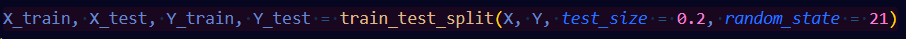
\includegraphics[width=1.0\linewidth]{split_data}
		\end{figure}
		
		
		\item Entraîner le modèle sur l'échantillon "\textit{train}": \\
		\textcolor{blue}{le modèle apprend le processus de génération des données, i.e, comment est-ce que les caractéristiques utilisées (prédicteurs ou \textit{features}) classifient les individus suivant la variable dépendante dans la catégorie 1 ou dans la catégorie 0}.
		\begin{figure}
			\centering
			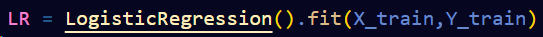
\includegraphics[width=0.7\linewidth]{train}
		\end{figure}
		
		
		\item  Tester le modèle en  évaluant  sa qualité prédictive. \\
		\textcolor{blue}{Dans quelle mesure est ce que le modèle a "bien appris" le processus de génération des valeurs de la variable cible?)}: \\
		\begin{itemize}
		\item		\textcolor{blue}{En pratique (par défaut), si $\widehat{Prob} (Y_i=1)>0.5$, on retient que l'individu concerné est classé par le modèle dans la catégorie 1 de la variable cible, étant données ses caractéristiques.}
		\end{itemize}
	\end{enumerate}
	
	
\end{frame}



\section{Qualité/performance}

\begin{frame}{Qualité/performance de l'exercice}
	\begin{enumerate}
	\item [1] Première approximation:  Matrice de confusion.
	
\end{enumerate}

	\begin{figure}
		\centering
		\includegraphics[width=0.7\linewidth]{qualité_adjust}
	\end{figure}
\end{frame}
	
	\begin{frame}{Qualité/performance de l'exercice}
		$\Rightarrow$ $\text{Count}-R^2=\dfrac{\text{nombre total d'estimations correctes }}{\text{nombre total d'estimations}}$\\
		% Pseudo R² supérieur à 70% est déjà pas mal
		
		\underline{Problème} : les valeurs des $y_i$ estimés sont comprises entre 0 et 1 mais seront la plupart du temps différentes des valeurs 0 et 1 $\Rightarrow$ à partir de quel seuil de $\widehat{y_i}$ peut on considérer que $\widehat{y_i}=1$ ? (pas de réponse universelle, généralement > 0.5).

\end{frame}

\begin{frame}
	\underline{Exemple} : 
	Soit  la matrice de confusion post estimation:
	% Please add the following required packages to your document preamble:
	% \usepackage[table,xcdraw]{xcolor}
	% If you use beamer only pass "xcolor=table" option, i.e. \documentclass[xcolor=table]{beamer}
	\begin{table}[]
		\begin{tabular}{|
				>{}c |c|c|}
			\hline
			\textbf{Observé/estimé} & \textbf{1} & \textbf{0} \\ \hline
			\textbf{1}              & 57                                 & 21                                 \\ \hline
			\textbf{0}              & 12                                 & 60                                 \\ \hline
		\end{tabular}
	\end{table}
	
	$\rightarrow$ A quoi est égal le count-$R^2$ ou  score de prédiction ou accuracy (exactitude).
	
	\pause 

$\text{Count}-R^2=\frac{57+60}{57+21+12+60}=\frac{117}{150}=0.78$

\vspace{0.5 cm}

\begin{enumerate}
	
 	\item[2] pseudo$R^2$ de Mc-Fadden  : $R^2_{MF}=1-\frac{ln(L_{NR})}{ln(L_R)}$\\
	Où :  $ln(L_{NR})$ est la fonction de log-vraissembleance dans le modèle non restreint (avec tous les régresseurs) et $ln(L_R)$ est la fonction de log-vraissemblance dans le modèle restreint (avec uniquement la constante $\beta_0$)
	% Si les régresseur n'expliquent rien alors les deux logs-vraissemblances sont égales et eur quotient est égal à 1 => R² de MF =1-1=0
	


\end{enumerate}
\end{frame}


\begin{frame}
	\begin{enumerate}
		
	\item [3] Différents taux d'intérêt (Précision, Recall ou Sensibilité, spécificité,... ) : Voir TP.

	\item[4] Receiver Operator Characteristic ROC, basé sur l'Area Under the Curve  (Air sous la Courbe)-AUC: \textit{taux de Vrais positifs} ou sensibilité en fonction du taux de  "faux positifs" (1-spécificité) à différents seuils de classement (Voir TP).

	
	\item[5] Validation croisée (non couvert)
	
	
\end{enumerate}


\end{frame}



\end{document}



\begin{frame}{Qualité de l'estimation}
	\underline{Test de significativité globale des coefficients} : 
	
	
	
	\underline{Hypothèses} : 
	\begin{itemize}
		\item $H_0$ : $\beta_0=\beta_1=\dots=\beta_k$
		
		\item $H_1$ Au moins un des coefficients est différent de 0
	\end{itemize}
	
	
	\underline{Statistique de test} : $LR=-2\left(ln(L_R)-ln(L_{NR})  \right) \sim \chi^2_{\alpha}(k)$
	
		
	\underline{Règle de décision} : Si $LR>\chi^2_{th, \alpha}(k)$ alors on rejette $H_0$ et on peut conclure qu'au moins un des coefficients est différent de 0.
	
\end{frame}

ROC curves typically feature true positive rate on the Y axis, and false positive rate on the X axis. This means that the top left corner of the plot is the “ideal” point - a false positive rate of zero, and a true positive rate of one. This is not very realistic, but it does mean that a larger area under the curve (AUC) is usually better.

The “steepness” of ROC curves is also important, since it is ideal to maximize the true positive rate while minimizing the false positive rate.

ROC curves are typically used in binary classification to study the output of a classifier. In order to extend ROC curve and ROC area to multi-label classification, it is necessary to binarize the output. One ROC curve can be drawn per label, but one can also draw a ROC curve by considering each element of the label indicator matrix as a binary prediction (micro-averaging).

Another evaluation measure for multi-label classification is macro-averaging, which gives equal weight to the classification of each label.

		\pause
\begin{comment}
	
	\item Dans ce modèle, la distribution des erreurs n'est plus normale. En effet, les erreurs ne peuvent prendre que deux valeurs  : 
	\begin{itemize}
		\item $\epsilon_i=0-\beta_0-\beta_1x_i$ 
		\item $\epsilon_i = 1-\beta_0-\beta_1x_i$
	\end{itemize}
	\item Les erreurs ne sont plus homoscédastiques : 
	\\
	$Var(\epsilon_i)=E(\epsilon_i^2)=p_i \times (1-\beta_0-\beta_1x_i)^2 + (1-p_i) \times (-\beta_0-\beta_1x_i)^2$\\
	$\Leftrightarrow$ $Var(\epsilon_i)=p_i(1-p_i)^2+(1-p_i)(p_i)^2$
	\\
	$\Leftrightarrow$ $Var(\epsilon_i)=p_i(1-p_i)$
\end{comment}


\begin{frame}{Modèle Probit}
	Dans la modélisation Probit, la fonction de répartition de $p_i$ est donnée par : 
	
	$$p_i=\int_{-\infty}^{\beta_0+\beta_1x_i}\frac{1}{\sqrt{2\pi}}e^{\frac{-t^2}{2}}dt $$
	
	$\Rightarrow$ Loi normale centrée-réduite
	
	On a  : 
	\pause
	\begin{itemize}
		\item$\lim\limits_{z_i \rightarrow +\infty} p_i=1$
		
		\vspace{0.4cm}
		\item $\lim\limits_{z_i \rightarrow -\infty} p_i=0$
	\end{itemize}
	
	Où : $z_i=\beta_0+\beta_1x_i$
\end{frame}
